\subsubsection{Struktura Ogólna Poziomu}
To tutaj kształtuje się świat gry, definiując główne obszary, trasy poruszania się gracza oraz punkty kluczowe. Zrozumienie tej struktury jest kluczowe dla zapewnienia płynności i logiczności rozgrywki. W tym kontekście, zajmiemy się analizą, jak zorganizować przestrzeń, aby stworzyć poziom, który nie tylko przyciąga wzrok, ale również dynamicznie reaguje na decyzje gracza.\\
W celu zapewnienia dynamiki naszemu poziomowi, postawiliśmy na rozwiązanie pozwalające uniknąć nadmiernego wczytywania - czyli umieszczenie wszystkich segmentów poziomu - w obrębie jednej sceny Unity.
Dodatkowo zastosowanie asynchronicznego ładowania sceny pozwoliło na stworzenie dużego poziomu bez większych problemów pod kątem wydajności.\\
Rozwiązanie to ma jednak swoje ograniczenia - utrudnia wprowadzanie zmian w scenie więcej niż jednej osobie ze względu na sposób przechowywania danych na temat sceny w jednym pliku - więc potencjalne jednoczesne wprowadzania zmian może prowadzić do niemożliwości otwarcia sceny/problemów przy commitach.
Wszelkie obiekty umieszczone na scenie znajdują się w hierarchii sceny tutaj:\\
\begin{figure}[h!]
    \centering
    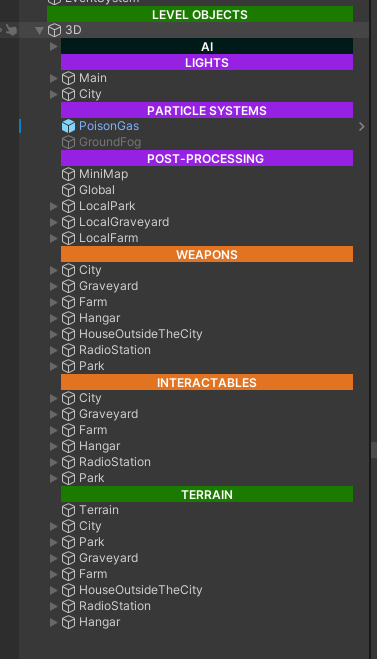
\includegraphics[width=0.41\linewidth]{Images/lvlhierarchy.png}
    \caption{Hierarchia obiektów na mapie}
    \label{fig:lvlhierarchy}
\end{figure}
\\Obiekty jak trawa, drzewa oraz kamienie dostępne są do edycji oraz rozmieszczania z poziomu ustawień terenu - to samo dotyczy wszelkich tekstur użytych do malowania podłoża:
\begin{figure}[h!]
    \centering
    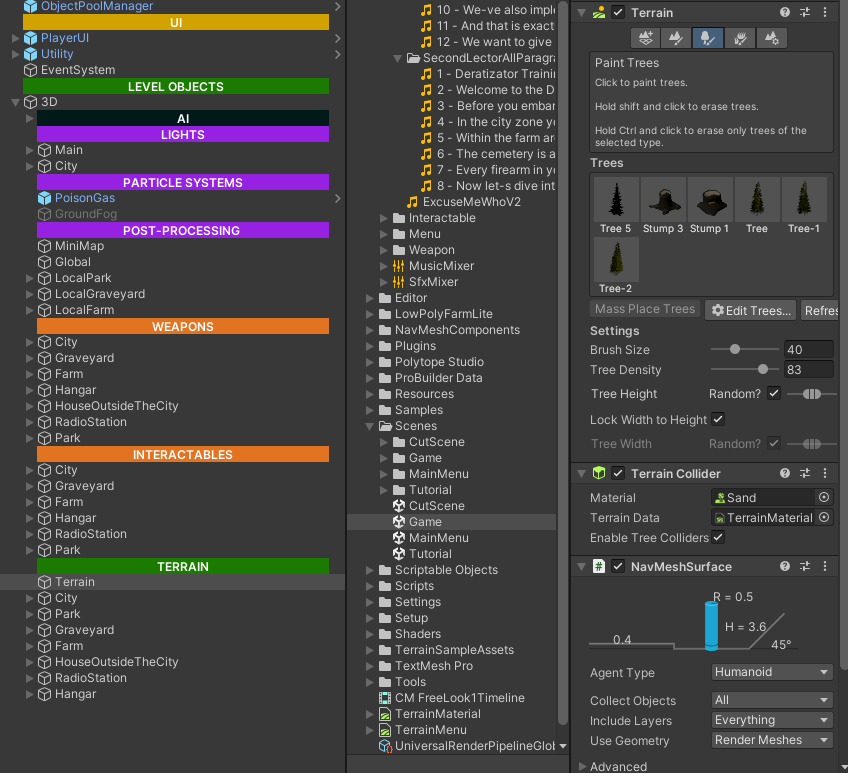
\includegraphics[width=0.65\linewidth]{Images/terrain.png}
    \caption{Ustawienia drzew na mapie - z poziomu terenu}
    \label{fig:enter-label}
\end{figure}
\begin{figure}[h!]
    \centering
    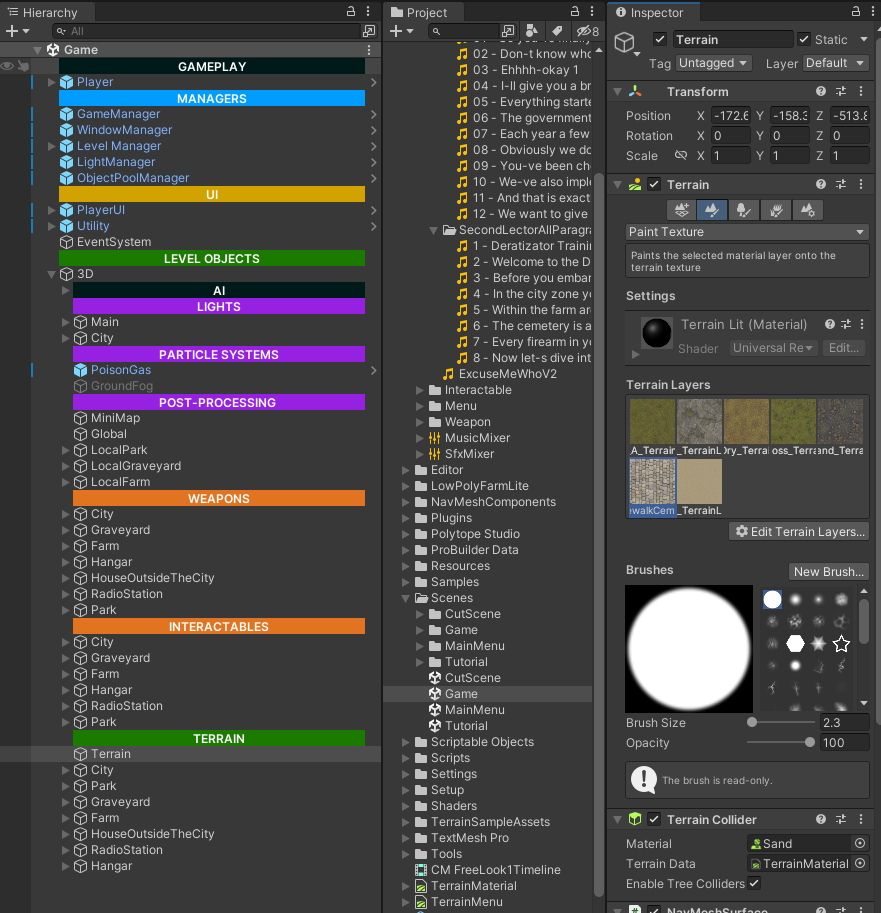
\includegraphics[width=0.65\linewidth]{Images/image.png}
    \caption{Użyte tekstury}
    \label{fig:enter-label}
\end{figure}
\newpage
\subsubsection{Sekcje i Obszary Kluczowe}
Poziom został podzielony na 4 główne sekcje, które wraz z postępami prac zostały rozdzielone na mniejsze obszary kluczowe.
Dodatkowo powstała również lokacja będąca łączeniem między sekcjami - w celu bardziej angażującej podróży pomiędzy owymi strefami - oraz makieta potencjalnej lokacji, która jednakże nie została wykorzystana - dostęp do niej jest zablokowany przez gaz - jednakże ze względu na aspekt wizualny (daje ona wrażenie że poza gazem również są tereny) została ona zachowana w obecnym scenariuszu
Strefy które możemy wyróżnić w grze to:
\begin{itemize}
    \item Cmentarz
    \item Miasto
    \item Farma
    \item Radiostacja
\end{itemize}
Wszystkie lokacje połączone są z sobą - dostep do nich jest nieograniczony - co daje graczowi dowolność w kolejności odwiedzania.

Wszystkie obiekty związane z danymi lokacjami są odpowiednio pogrupowane w celu ułatwienia nawigacji przy potencjalnym wprowadzaniu zmian:
\begin{figure}[h]
    \centering
    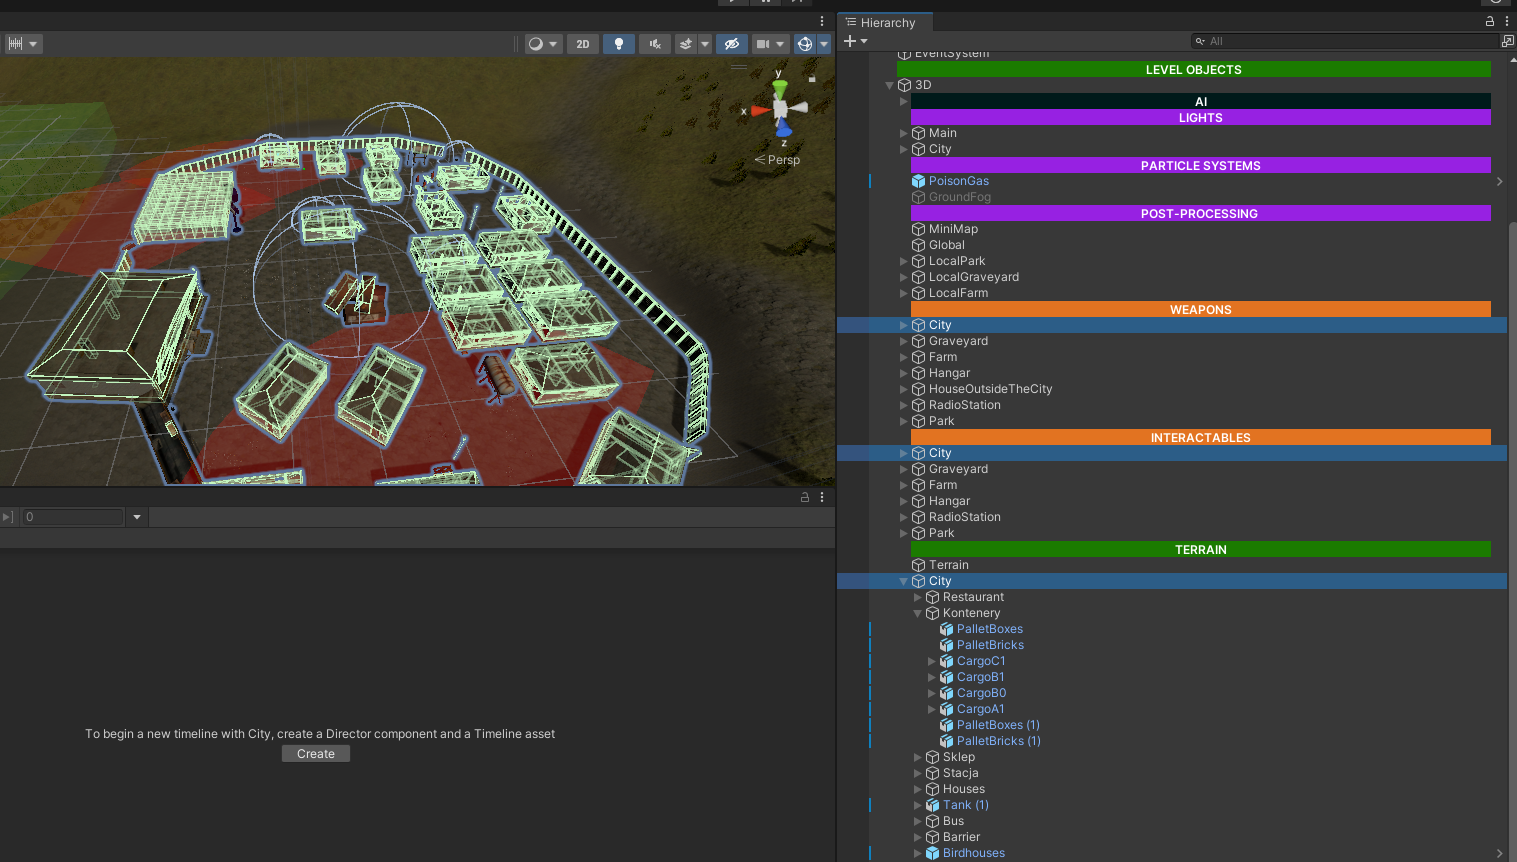
\includegraphics[width=1\linewidth]{Images/cityexamplehierarchy.png}
    \caption{Przykład hierarchii dla sekcji miasta}
    \label{fig:enter-label}
\end{figure}
Każda z sekcji jest również rozbita na obszary kluczowe dla niej - główne punkty uwagi gracza, które będą najczęściej odwiedzane
Są to:
\begin{itemize}
    \item Dla miasta są to:
    \begin{itemize}
        \item Restauracja
        \item Stos kontenerów na środku
        \item Wrak autobusu
        \item Sklep
        \item Sekcja domków szeregowych - 7 identycznych domów w rzędach
        \item Stacja benzynowa
    \end{itemize}
    \item Sekcja cmentarza jest podzielona na:
    \begin{itemize}
        \item Sekcja wejściowa- brama praz nagrobki
        \item Sekcja środkowa - ołtarz oraz kolumny
        \item Sekcja tylnia- kurhany, mniejszy wydzielony fragment z nagrobkami
    \end{itemize}
    \item Farma została podzielona na
    \begin{itemize}
        \item Sekcja domów
        \item Pola uprawne
    \end{itemize}
    \item Radiostacja posiada następujące punkty zainteresowania:
    \begin{itemize}
        \item Budynek Radiostacji
        \item Kontenery z skrzyniami
    \end{itemize}
\end{itemize}

Taki rozkład znacznie ułatwiał pracę nad poszczególnymi lokacjami - każdy z punktów kluczowych został osobno zaprojektowany i wdrożony, następnie połączenie ich dawało praktycznie gotową lokację.
\subsubsection{Połączenia Między Sekcjami}

Połączenia między sekcjami muszą być zarówno interesujące pod kątem posiadanej zawartości - jak również wizualnie.
Jednocześnie w dalszym ciągu powinny być łatwo widoczne oraz intuicyjne dla gracza.
Ze względu na rozmiar mapy  jak i zastosowanie minimapy intuicyjność wyboru ścieżki i miejsca dokąd prowadzi nie stanowi żadnego wyzwania pod kątem tworzenia poziomu - gdyż lokacje są widoczne.\\
W ramach zachęty do stosowania przez gracza wytyczonych ścieżek - pozostałe trasy posiadają dużą ilość drzew.
Powoduje to znaczne spowolnienie w przemierzaniu terenu - jednakże gwarantuje większą ochronę - gdyż drzewa posiadają collidery, co sprawia że pocisk wystrzelony w strone gracza może zatrzymać się na obiekcie drzewa.\\
Zastosowane w grze ściezki zostały wykonane przez naniesienie odpowiedniej, różnej od pozostałej powierzchni, tekstury - by za pomocą skojarzeń z dnia codziennego przekazać informacje "to jest ścieżka" graczowi.
\begin{figure}[h]
    \centering
    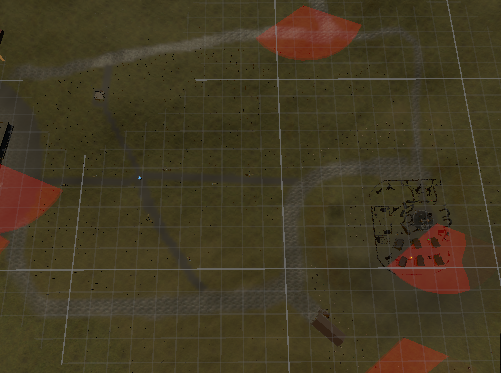
\includegraphics[width=0.5\linewidth]{Images/paths.png}
    \caption{Sciezki naniesione na teren za pomoca tekstury}
    \label{fig:enter-label}
\end{figure}

W celu urozmaicenia podróży gracza, na przecięciu najważniejszych ścieżek prowadzących do głównych sekcji wymienionych wyżej, została wprowadzona nowa podlokacja - Park.
Umieszczenie kilku ławek, koszy oraz latarnii z dodaną emisją sprawiło że ścieżka nie sprawia wrażenie pustej, świat wydaje się żywszy i realniejszy.
Dodatkowo gracz może znaleźć po drodze na kilka broni - co okazało się konieczne w sytuacjach gdzie AI w agresywny sposób wykorzystało dostępne na mapie zasoby i zmusiło gracza do ucieczki - pozwoliło to uniknąć sytuacji gdzie gracz ginie bez możliwości sensownej obrony.

Warto również wspomnieć że wszelkie lokalizacje mijane po drodze posiadają również teleportery, będace punktami startowymi dla gracza oraz botów. Poszczególne lokacje posiadają różne warianty kolorystyczne owych teleporterów, co może być swego rodzaju informacją dla gracza dzięki dobraniu kolorów powodującym skojarzenia:
\begin{itemize}
    \item Cmentarz \& kościół - pomarańczowy
    \item Radiostacja \& okolice - niebieski
    \item Farma - żółty
    \item Park\& okolice lasu między lokacjami - zielony
    \item Miasto - różowy
\end{itemize}